\documentclass[xcolor=pdftex,dvipsnames,table,aspectratio=169]{beamer}
%\documentclass[xcolor=pdftex,dvipsnames,table,handout,aspectratio=169]{beamer}

%\setbeameroption{show notes}

\usepackage{bm,graphicx,multirow,amsmath,tikz} %fancybox,
\usepackage{color}%,textpos}
\usepackage[round]{natbib}
\usepackage[normalem]{ulem}
\usepackage{hyperref}
\usepackage{lastpage}
\usepackage{array}
\usepackage{color}
\usepackage{framed}
\usepackage{hyperref}

% Define Western colours
\definecolor{western}{rgb}{.306,.152,.524}
\definecolor{westerngray}{rgb}{.512,.508,.524}

%% Define BEAMER colours
\setbeamercolor{frametitle}{bg=western,fg=white}
\setbeamercolor{framesubtitle}{bg=western,fg=black}
\setbeamercolor{title}{fg=white,bg=western}
\setbeamercolor{author}{fg=white,bg=western}
\setbeamercolor{institute}{fg=white,bg=western}
\setbeamercolor{date}{fg=white,bg=western}

%% Set BEAMER fonts
\setbeamerfont{title}{shape=\bf}
\setbeamerfont{frametitle}{shape=\sc,size=\Large}
\setbeamerfont{framesubtitle}{shape=\sc,size=\Large}
\setbeamerfont{footline}{shape=\sc}

%% Define BEAMER toc
\setbeamercolor{section in toc}{fg=western}
\setbeamercolor{subsection in toc}{fg=westerngray}
\setbeamertemplate{sections/subsections in toc}[ball]

%% Define BEAMER background
\setbeamercolor{background canvas}{bg=white}

%% Define BEAMER footer
\setbeamertemplate{navigation symbols}{}
\setbeamercolor{footline}{fg=white,bg=western}
\setbeamertemplate{footline}{%
  \begin{beamercolorbox}[wd=\paperwidth]{footline}
    \vskip5pt

    \raisebox{.05in}{
      \scriptsize{\bf \insertshorttitle}
    }
    \hfill
    \raisebox{.05in}{
      \scriptsize{\bf \insertframenumber/\inserttotalframenumber} 
    }
    \hspace{5pt}

    \vskip5pt
  \end{beamercolorbox}
}

%% Define BLOCK environment
\setbeamercolor{block title}{fg=western}
\setbeamerfont{block title}{series=\bfseries}

%% Define ENUMERATE and ITEMIZE environements
\setbeamertemplate{itemize item}[ball]
\setbeamertemplate{enumerate item}[ball]
\setbeamercolor{item projected}{bg=western}

%% Define BEAMER toc
\setbeamercolor{sections/subsections in toc}{fg=blue!75}
\setbeamertemplate{sections/subsections in toc}[ball]

% %% Define SECTION openings
% \AtBeginSection[]{
%   \begin{frame}{\insertshorttitle}
%     \tableofcontents[currentsection,subsectionstyle=hide/hide/hide]
    
%   \end{frame}
% }

%% Define BEAMER frametitle
\addtobeamertemplate{frametitle}{
   \let\insertframetitle\insertsectionhead}{}
\addtobeamertemplate{frametitle}{
   \let\insertframesubtitle\insertsubsectionhead}{}


\makeatletter
  \CheckCommand*\beamer@checkframetitle{\@ifnextchar\bgroup\beamer@inlineframetitle{}}
  \renewcommand*\beamer@checkframetitle{\global\let\beamer@frametitle\relax\@ifnextchar\bgroup\beamer@inlineframetitle{}}
\makeatother

% Define counters for example and exercise
\newcounter{example}
\newcounter{exercise}

% Define example and exercise commands
\renewcommand{\example}
{\stepcounter{example}Example \lecturenum.\arabic{example}}
\newcommand{\examplectd}
{Example \lecturenum.\arabic{example}\ ctd}
\newcommand{\exercise}
{\stepcounter{exercise}Exercise \lecturenum.\arabic{exercise}}
\newcommand{\exercisectd}
{Exercise \lecturenum.\arabic{exercise}\ ctd}

\newcommand{\lecturenum}{12}

\title[SS2857]{Probability and Statistics I}
\subtitle{\lecturenum. The Poisson Distribution}

\date{}

%% Add logo
%% \titlegraphic{\includegraphics[height=2cm]{../uwo_logo_reversed}}

%% Initialize R


\begin{document}

{
\setbeamertemplate{footline}{}
\setbeamercolor{background canvas}{bg=western}

\begin{frame}
  \addtocounter{framenumber}{-1}

  \maketitle
\end{frame}
}

\begin{frame}
  \frametitle{\invisible{Hello}}

  \begin{center}
    
    \Large{\textbf{3.7 The Poisson Distribution}}
  \end{center}
  
  
  \begin{center}
    
\includegraphics[height=.5\textheight]{figure/umbrella}
  \end{center}



\end{frame}

\section{The Poisson Distribution}

\begin{frame}
  \begin{block}{The Poisson Distribution}
  We say that $X$ has a Poisson distribution with mean $\lambda$ if $X$ has pmf
  $$
  P(X=x)=p(x;\lambda)=\frac{e^{-\lambda} \lambda^x}{x!},\quad x=0,1,2,\ldots.
  $$
  
  \medskip
  
  Mathematically
      \[
        X \sim \mbox{Poisson}(\lambda).
      \]
  \end{block}
\end{frame}

\begin{frame}
  \begin{block}{PMF and CDF}
    \begin{itemize}
    \item PMF: $p(x;\lambda)=\frac{e^{-\lambda}\lambda^x}{x!},\quad x=0,1,2,\ldots$.
    \item CDF: requires special functions
    \end{itemize}
  \end{block}

  %\begin{block}{Moment Generating Function}
  %  \[
  %    M_X(t)=e^{\lambda(e^t-1)}
  %  \]
  %\end{block}

  \begin{block}{Properties}
    \begin{itemize}
    \item Mean: $E(X)=\lambda$
      
    \item Variance: $V(X)=\lambda$
      
   % \item Skewness: $\lambda^{-1/2}$
    \end{itemize}
  \end{block}
\end{frame}

\begin{frame}
  \begin{block}{The Poisson Distribution}
    The Poisson distribution is most commonly used to model the number of times a specific event occurs within a fixed time period or the number of items in a fixed area.
    
    \medskip
    
    E.g.:
    \begin{itemize}
    \item The number of patients admitted to hospital in a day.
    \item The number of goals a soccer player scores in a season.
    \item The number of claims to an insurance company in a year.
    \item the number of students in a class. 
    \end{itemize}
  \end{block}

\end{frame}

\begin{frame}
  \begin{block}{Poisson Process}
  \only<1-4>{
    \begin{enumerate}
    \item The probability of exactly one event in a short time interval of length $\Delta t$ tends toward $\alpha \Delta t$ as $\Delta t$ decreases.
    \item The probability of exactly zero events in a short time interval of length $\Delta t$ tends toward $1-\alpha \Delta t$ as $\Delta t$ decreases.
    \item The number of events in disjoint intervals are independent.
    \end{enumerate}
  }
  
  \only<2>{
  \medskip
  Points 1 and 2 imply:
  \begin{itemize}
  \item the rate of events is constant, $\alpha$ events per unit time on average.
  \item events cannot occur simultaneously.
  \end{itemize}
  }

    \only<3>{
      Under these conditions, the number of events in an interval of length 1 has a Poisson distribution with parameter $\lambda=\alpha$.

      \bigskip
      Mathematically
      \[
        X \sim \mbox{Poisson}(\alpha).
      \]
    }
    \only<4>{
      Under these conditions, the number of events in an interval of length $t$ has a Poisson distribution with parameter $\alpha t$.

      \bigskip
      Mathematically
      \[
        X \sim \mbox{Poisson}(\alpha t).
      \]
    }

  \end{block}
\end{frame}

\begin{frame}
  \begin{block}{\example}
    According to the book ``United States Water Law: An Introduction'' by John W.~Johnson, heavy rain falls at about 495 drops per second per metre square. Let $X$ be the number of rain drops that falls in one metre square in $t$ seconds.
    \begin{enumerate}[a)]
    \item What is the distribution of $X$?
    \item What is the pmf of $X$?
    \item What are the mean and variance of $X$?
    \item How does the shape of the distribution vary with $t$?
    \end{enumerate}
  \end{block}
\end{frame}




\begin{frame}
  \begin{block}{\examplectd}
% latex table generated in R 4.4.1 by xtable 1.8-4 package
% Wed Oct  9 11:51:19 2024
\begin{table}[ht]
\centering
\begin{tabular}{rrr}
  \hline
t & Mean & Variance \\ 
  \hline
0.001 & 0.495 & 0.495 \\ 
  0.010 & 4.950 & 4.950 \\ 
  0.100 & 49.500 & 49.500 \\ 
  1.000 & 495.000 & 495.000 \\ 
   \hline
\end{tabular}
\end{table}

  \end{block}
\end{frame}

\begin{frame}
  \begin{block}{\examplectd}
    \begin{center}
      \begin{tabular}{cc}
        $t=0.001$
        &$t=0.01$
        \\
        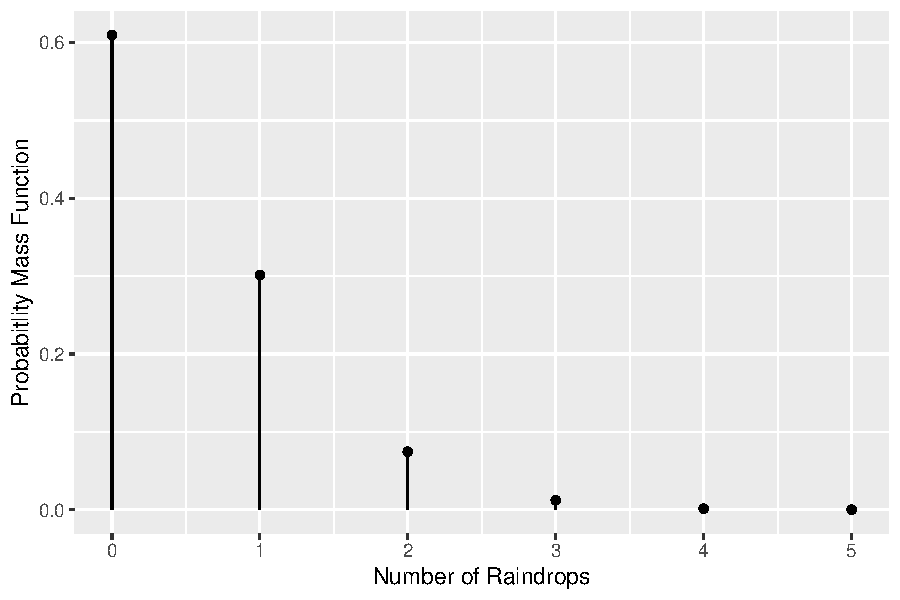
\includegraphics[width=.4\textheight]{figure/rainfall-1}
        & 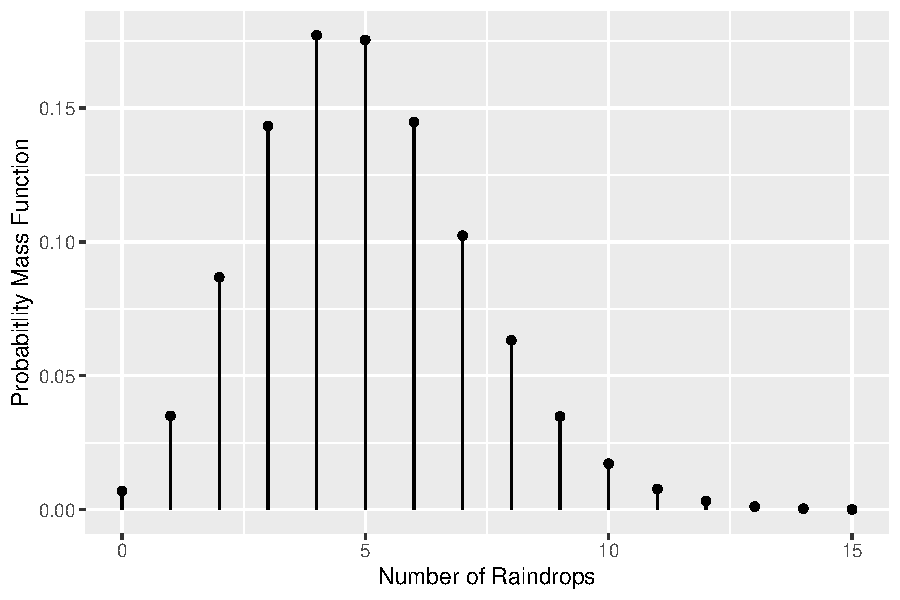
\includegraphics[width=.4\textheight]{figure/rainfall-2} \\
        $t=0.1$
        &$t=1$
        \\
        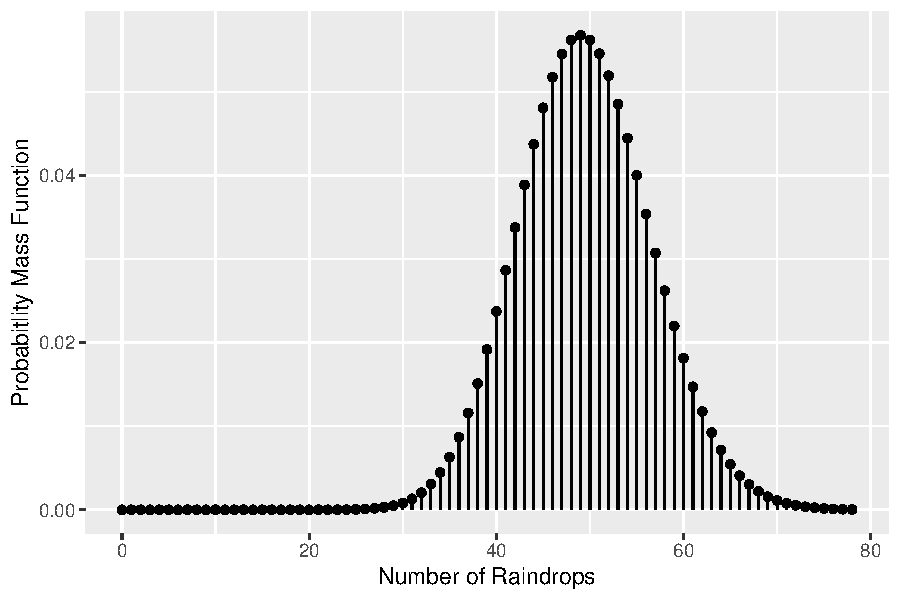
\includegraphics[width=.4\textheight]{figure/rainfall-3}
        & 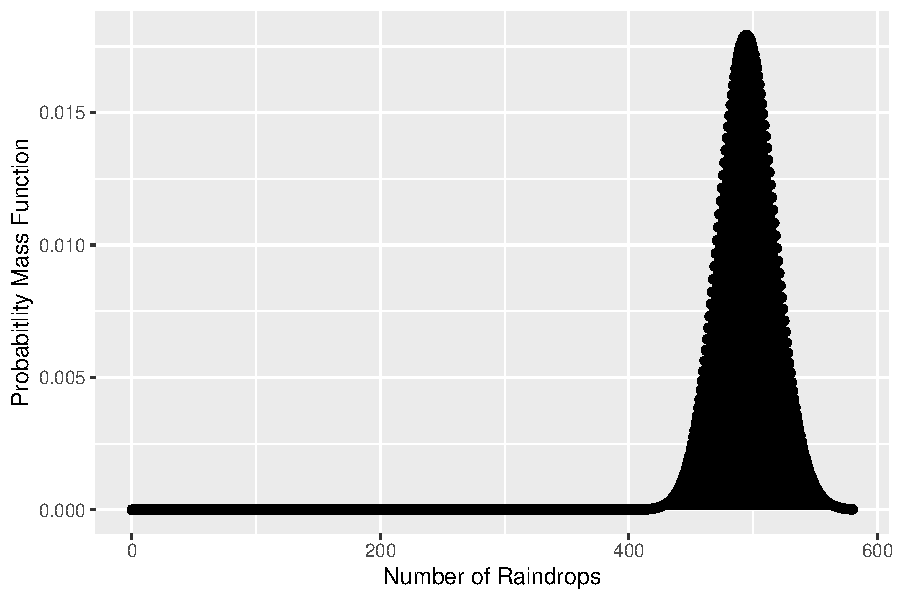
\includegraphics[width=.4\textheight]{figure/rainfall-4} \\
      \end{tabular}
    \end{center}
  \end{block}
\end{frame}

\begin{frame}

  \begin{block}{Poisson Approximation to the Binomial}
  
  Suppose that
  $$
  X \sim \mbox{Binomial}(n,p)
  $$
  such that $n$ is large and $\mu_X=np$ is small\footnote{Your book uses the rule of thumb $n>50$ and $np<5$}. 
  
  \medskip
  Then we can approximate the distribution of $X$ with a Poisson distribution
  $$
  X \overset{\cdot}{\sim} \mbox{Poisson}(np).
  $$
  
  \end{block}
\end{frame}

\begin{frame}

  \begin{block}{\example}
  In lecture 4, we showed that the probability that a randomly selected person is colour blind is about .04512. Let $X$ be the number of colour blind students in a class of 100.
  
  \begin{enumerate}[a)]
  \item What is the distribution of $X$?
  \item What are the mean and variance of $X$?
  \item What is the probability that the class contains more than 5 students who are colour blind?
  \item Approximate the distribution of $X$ by a Poisson and repeat the questions above. 
  \item Do you think the Poisson approximation is appropriate?
  \end{enumerate}
  
  \end{block}
\end{frame}

\begin{frame}
  \begin{center}
    \Large{\textbf{Questions?}}
  \end{center}
\end{frame}

\begin{frame}
  \begin{block}{\exercise}
  One gram of Uranium-235 contains $2.35 \times 10^{21}$ atoms. Each atom has probability $9.85 \times 10^{-10}$ of decaying in one year. Let $X$ be the number of atoms that decay in 1 year. You may assume that atoms decay independently of one another.
  
  \begin{enumerate}[a)]
  \item What is the distribution of $X$?
  \item What are the mean and variance of $X$?
  \item What is the probability that the number of decays in one year is greater than the mean?
  \item Approximate the distribution of $X$ by a Poisson and repeat the questions above. 
  \item Do you think the Poisson approximation is appropriate?
  \end{enumerate}
  \end{block}
\end{frame}

\end{document}

